\begin{figure}[H]
  \begin{center}
    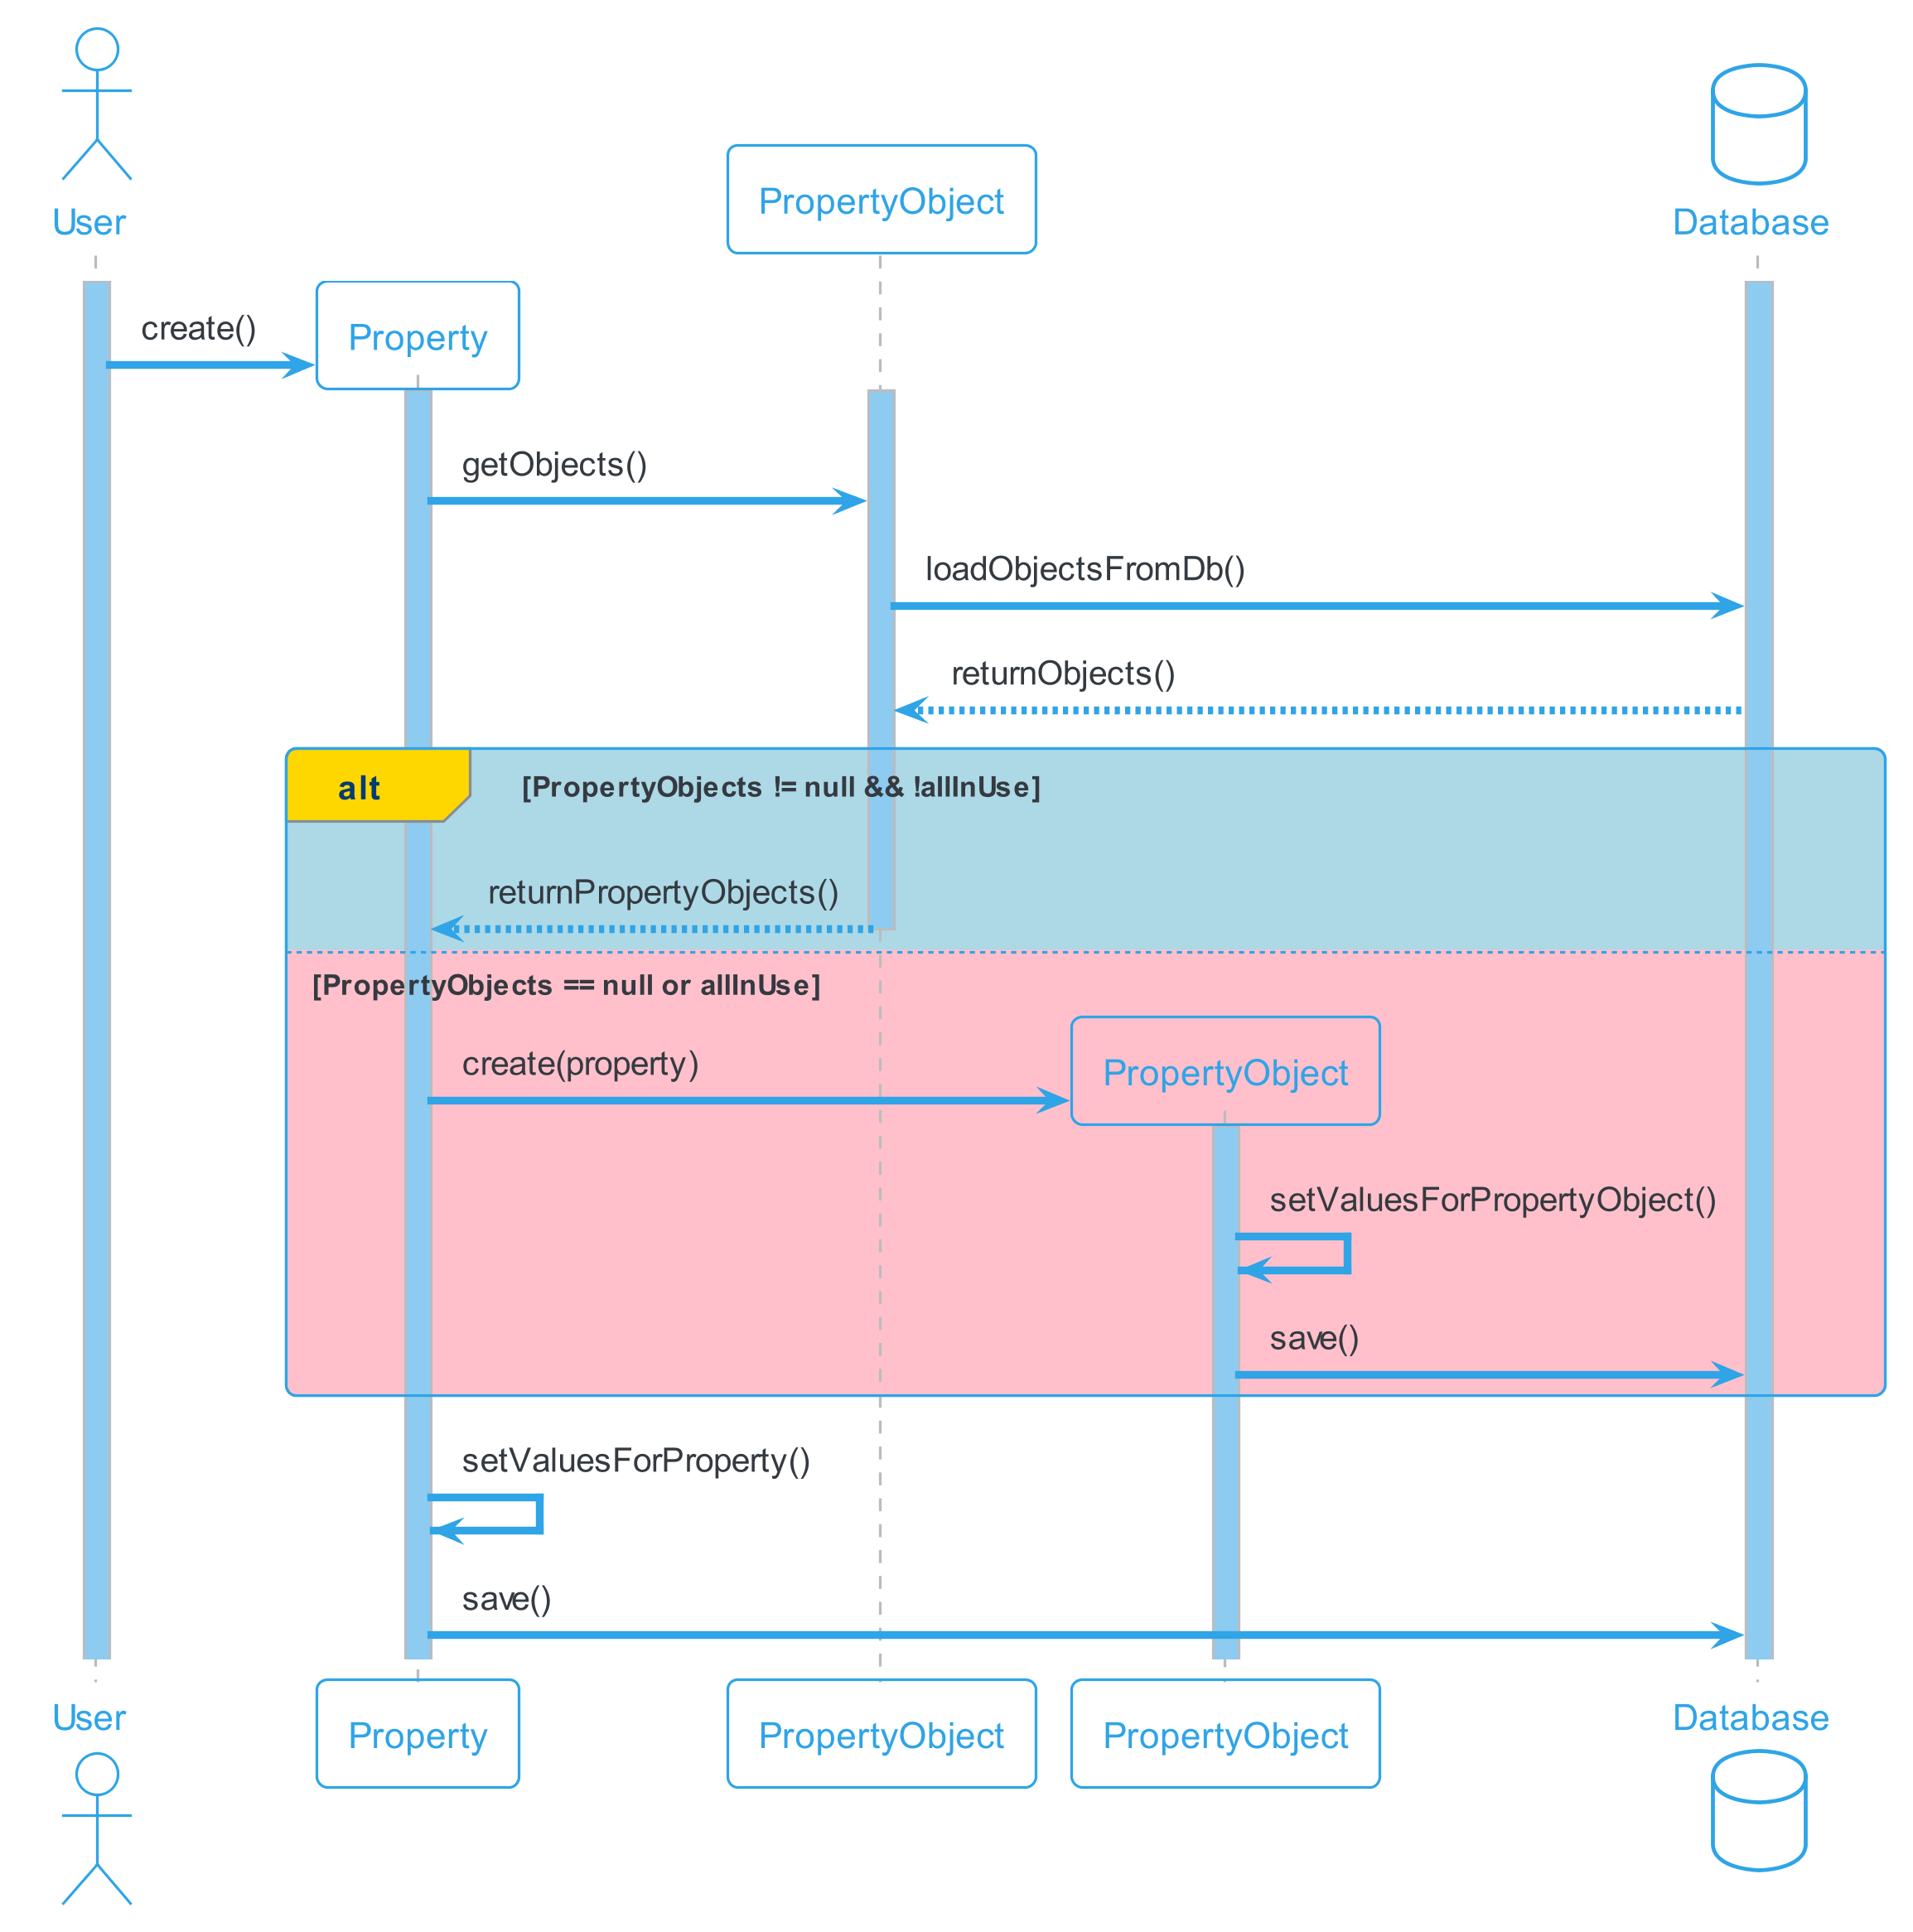
\includegraphics[width=0.55\linewidth]{content/diagrams/out/sequenzdiagram/liegenschaftErfassen/LiegenschaftErfassen.png}
    \caption{SQ-Liegenschaft erfassen}
  \end{center}
\end{figure}

\begin{figure}[H]
  \begin{center}
    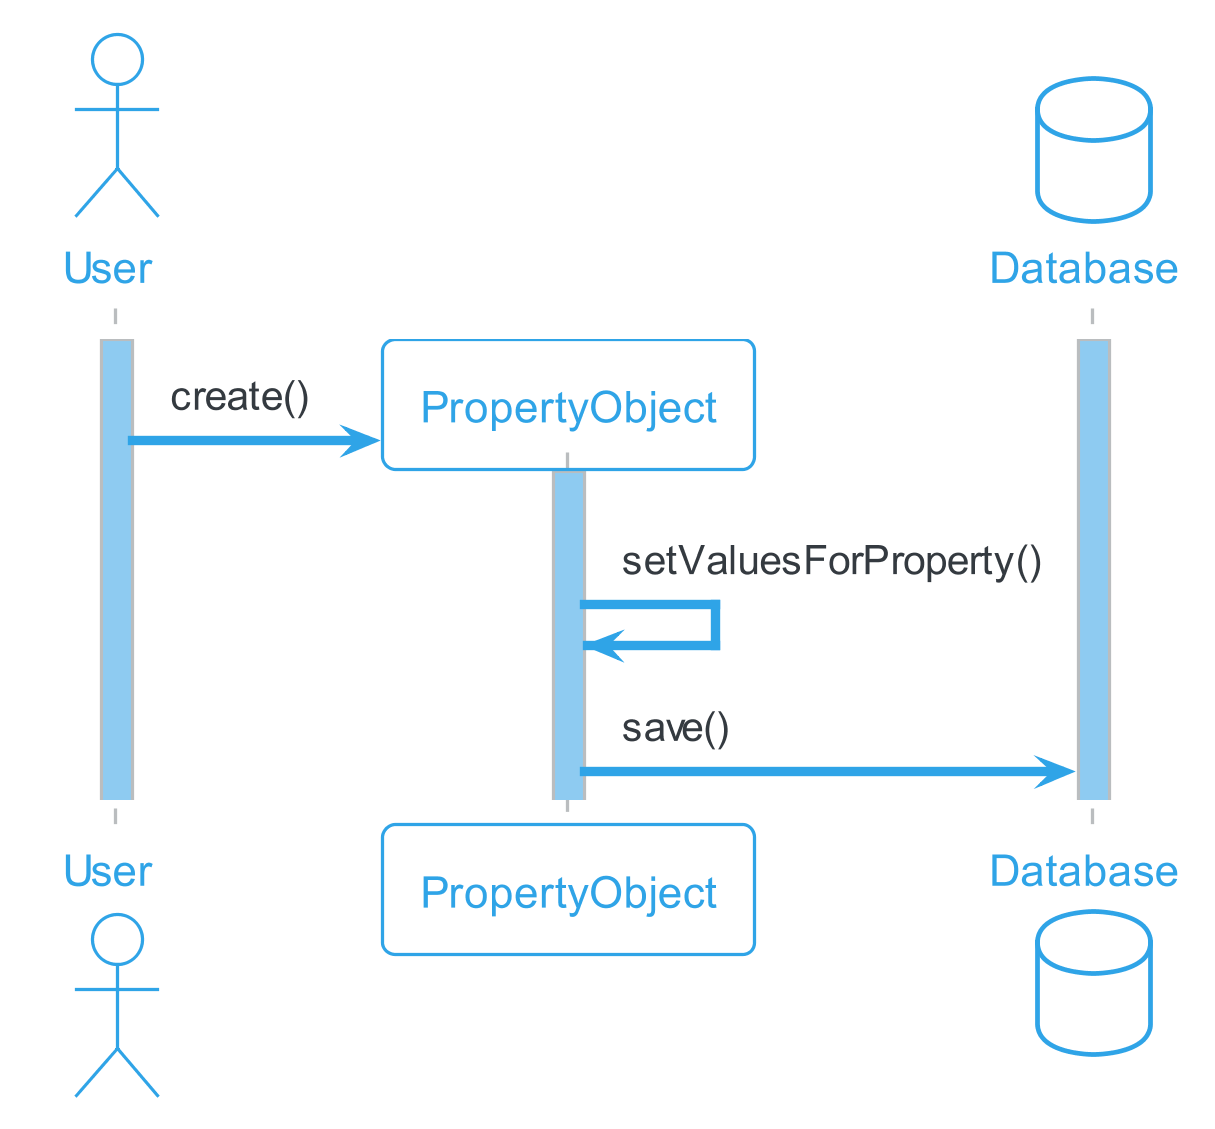
\includegraphics[width=0.55\linewidth]{content/diagrams/out/sequenzdiagram/objektErfassen/ObjekttErfassen.png}
    \caption{SQ-Objekt erfassen}
  \end{center}
\end{figure}

\begin{figure}[H]
  \begin{center}
    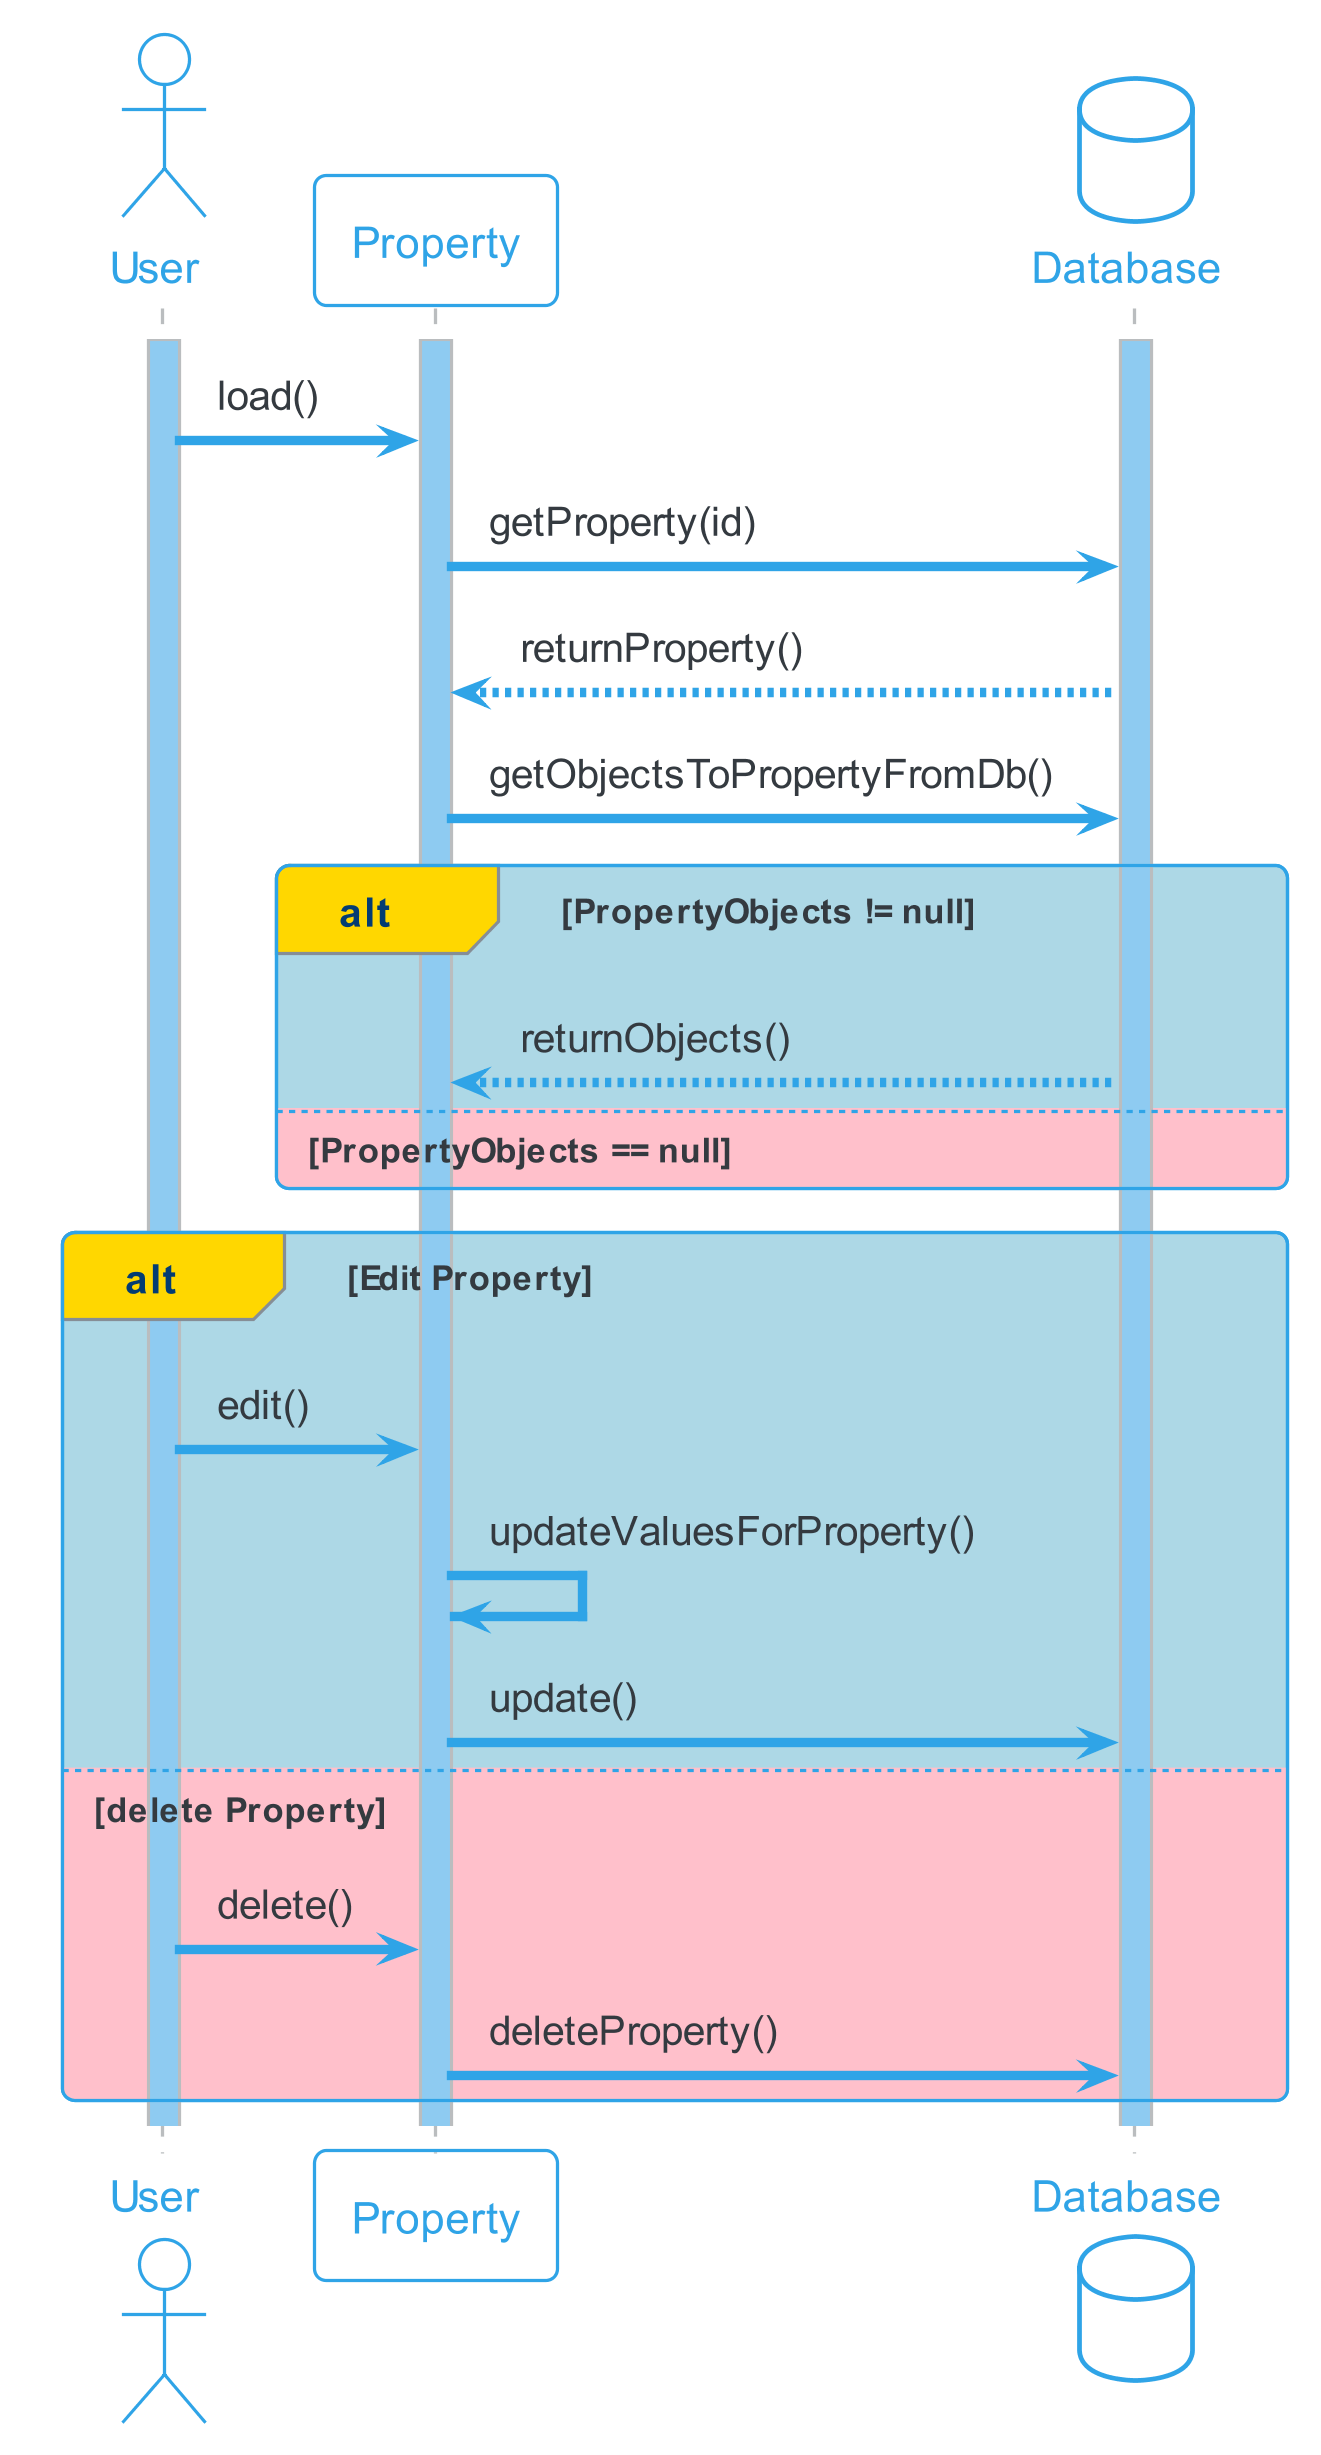
\includegraphics[width=0.5\textheight]{content/diagrams/out/sequenzdiagram/liegenschaftAnsehenBearbeiten/LiegenschaftAnsehenBearbeiten.png}
    \caption{SQ-Liegenschaft Ansehen / Bearbeiten / Löschen}
  \end{center}
\end{figure}

\begin{figure}[H]
  \begin{center}
    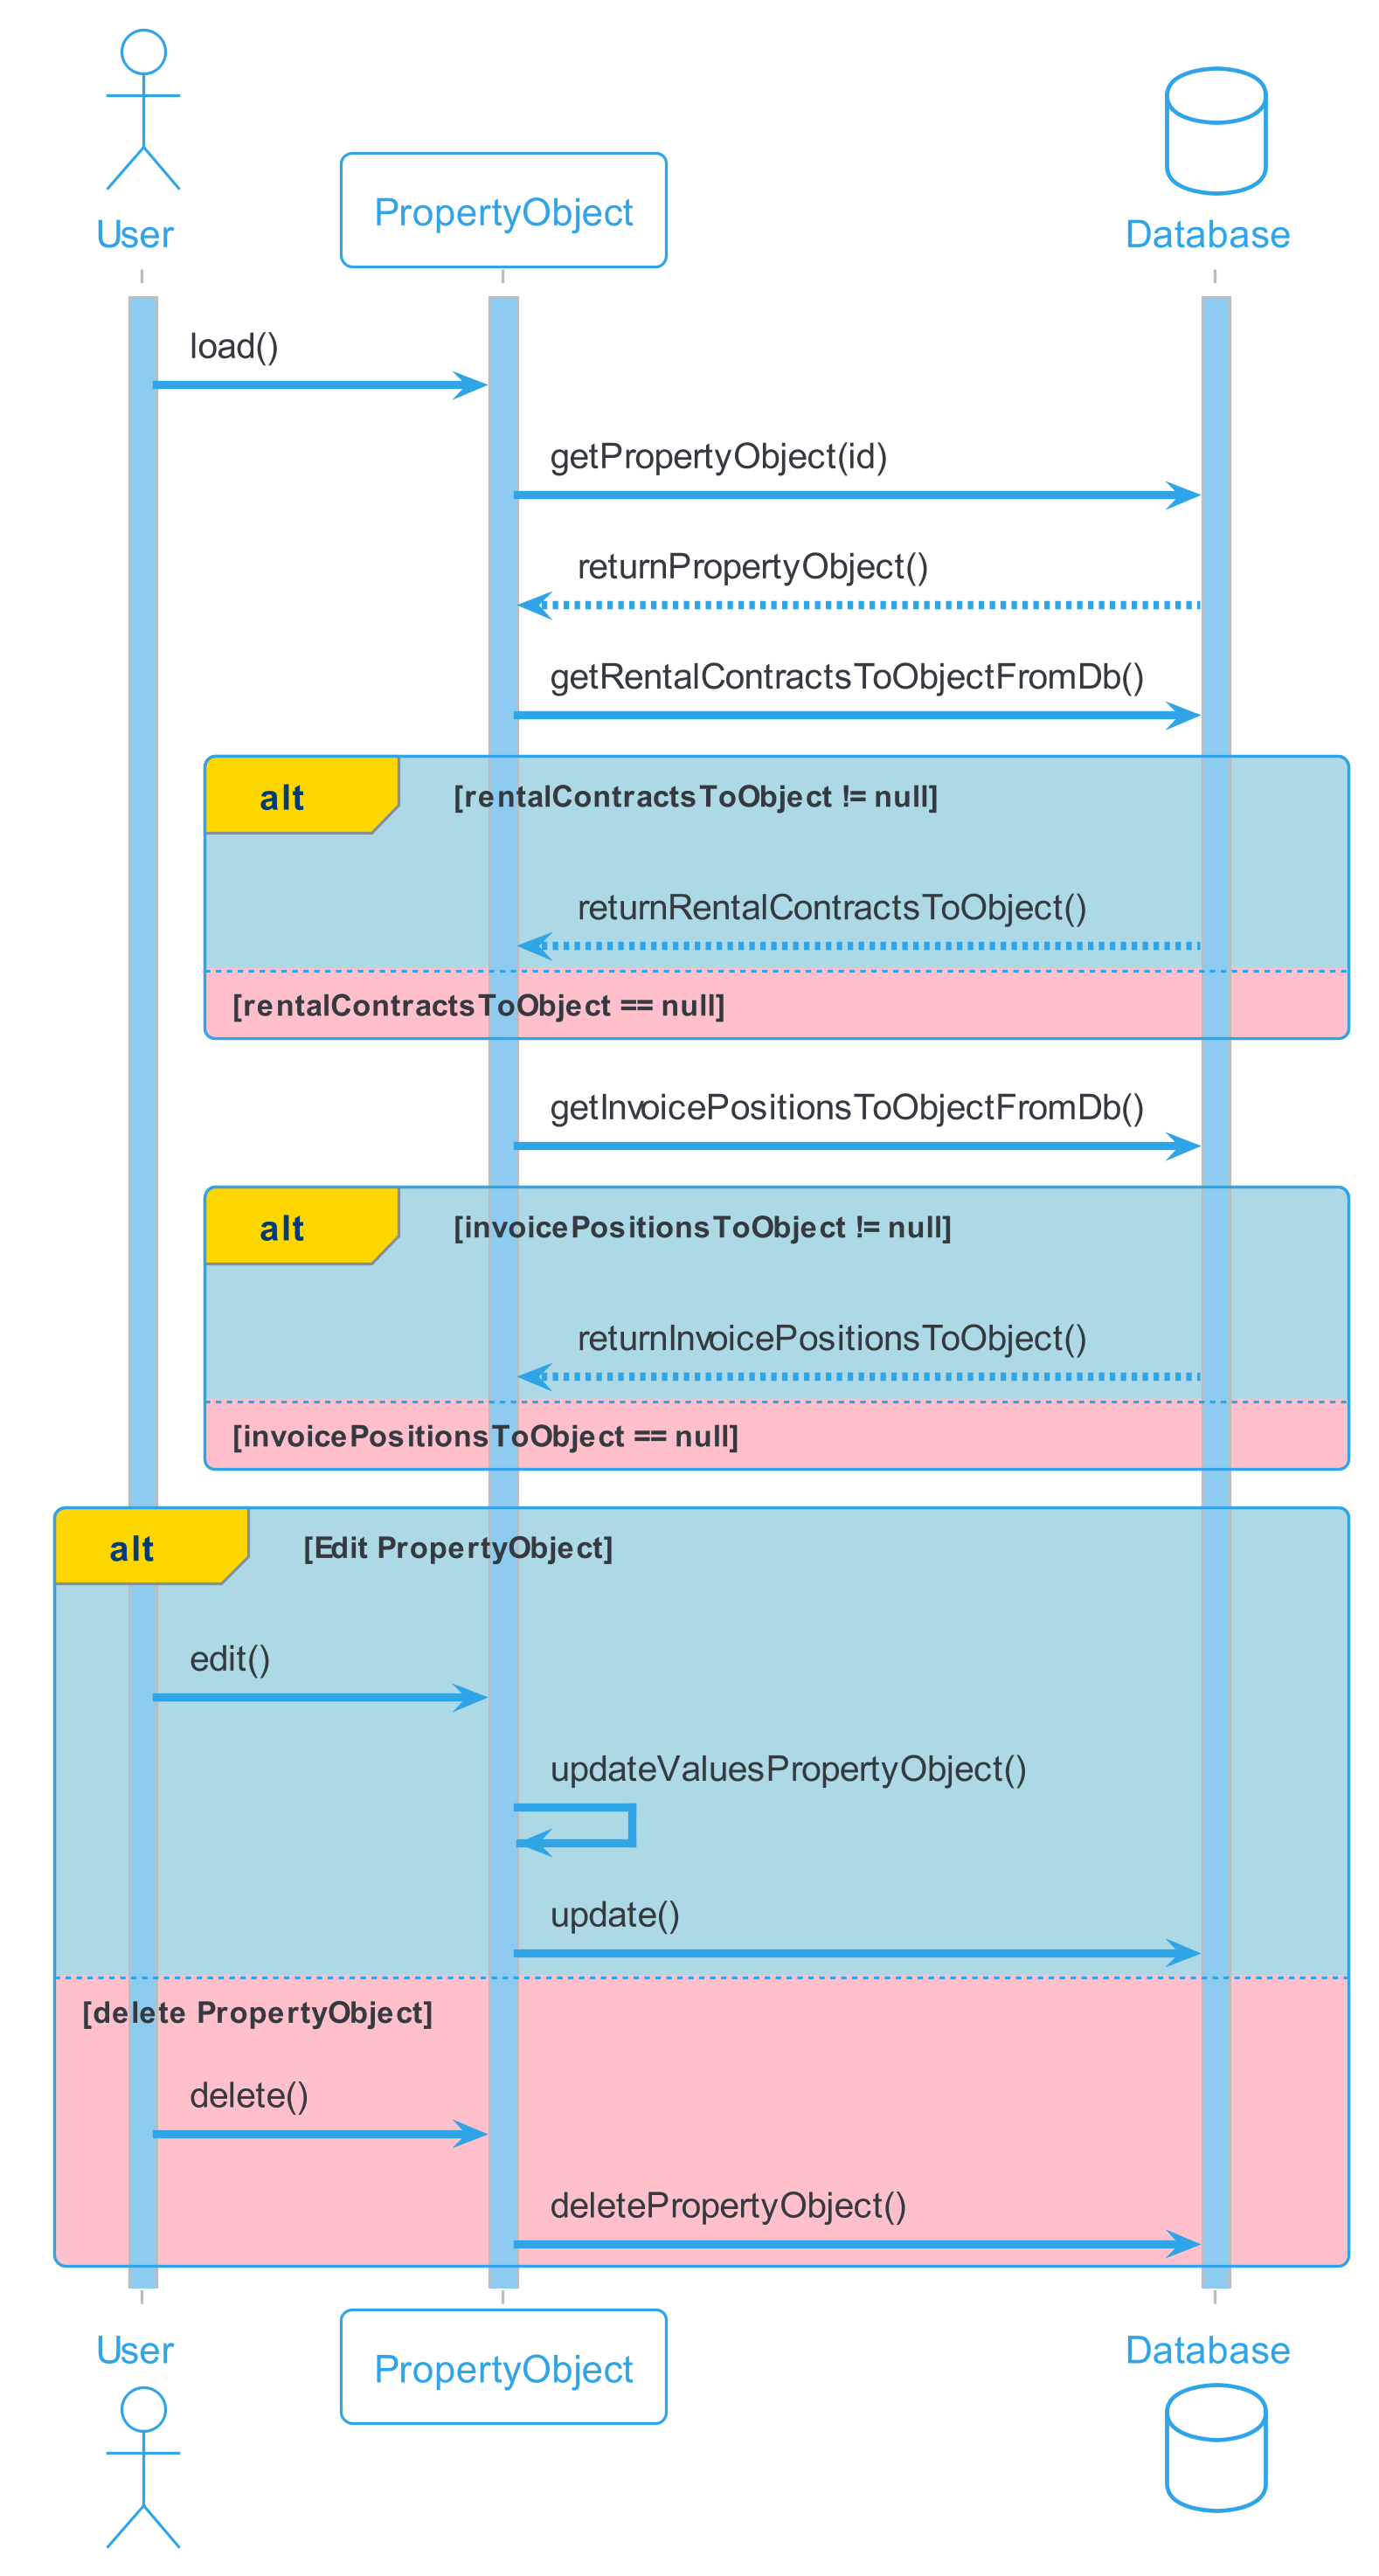
\includegraphics[width=0.5\textheight]{content/diagrams/out/sequenzdiagram/objektAnsehenBearbeiten/objektAnsehenBearbeiten.png}
    \caption{SQ-Objekt Ansehen / Bearbeiten / Löschen}
  \end{center}
\end{figure}

\begin{figure}[H]
  \begin{center}
    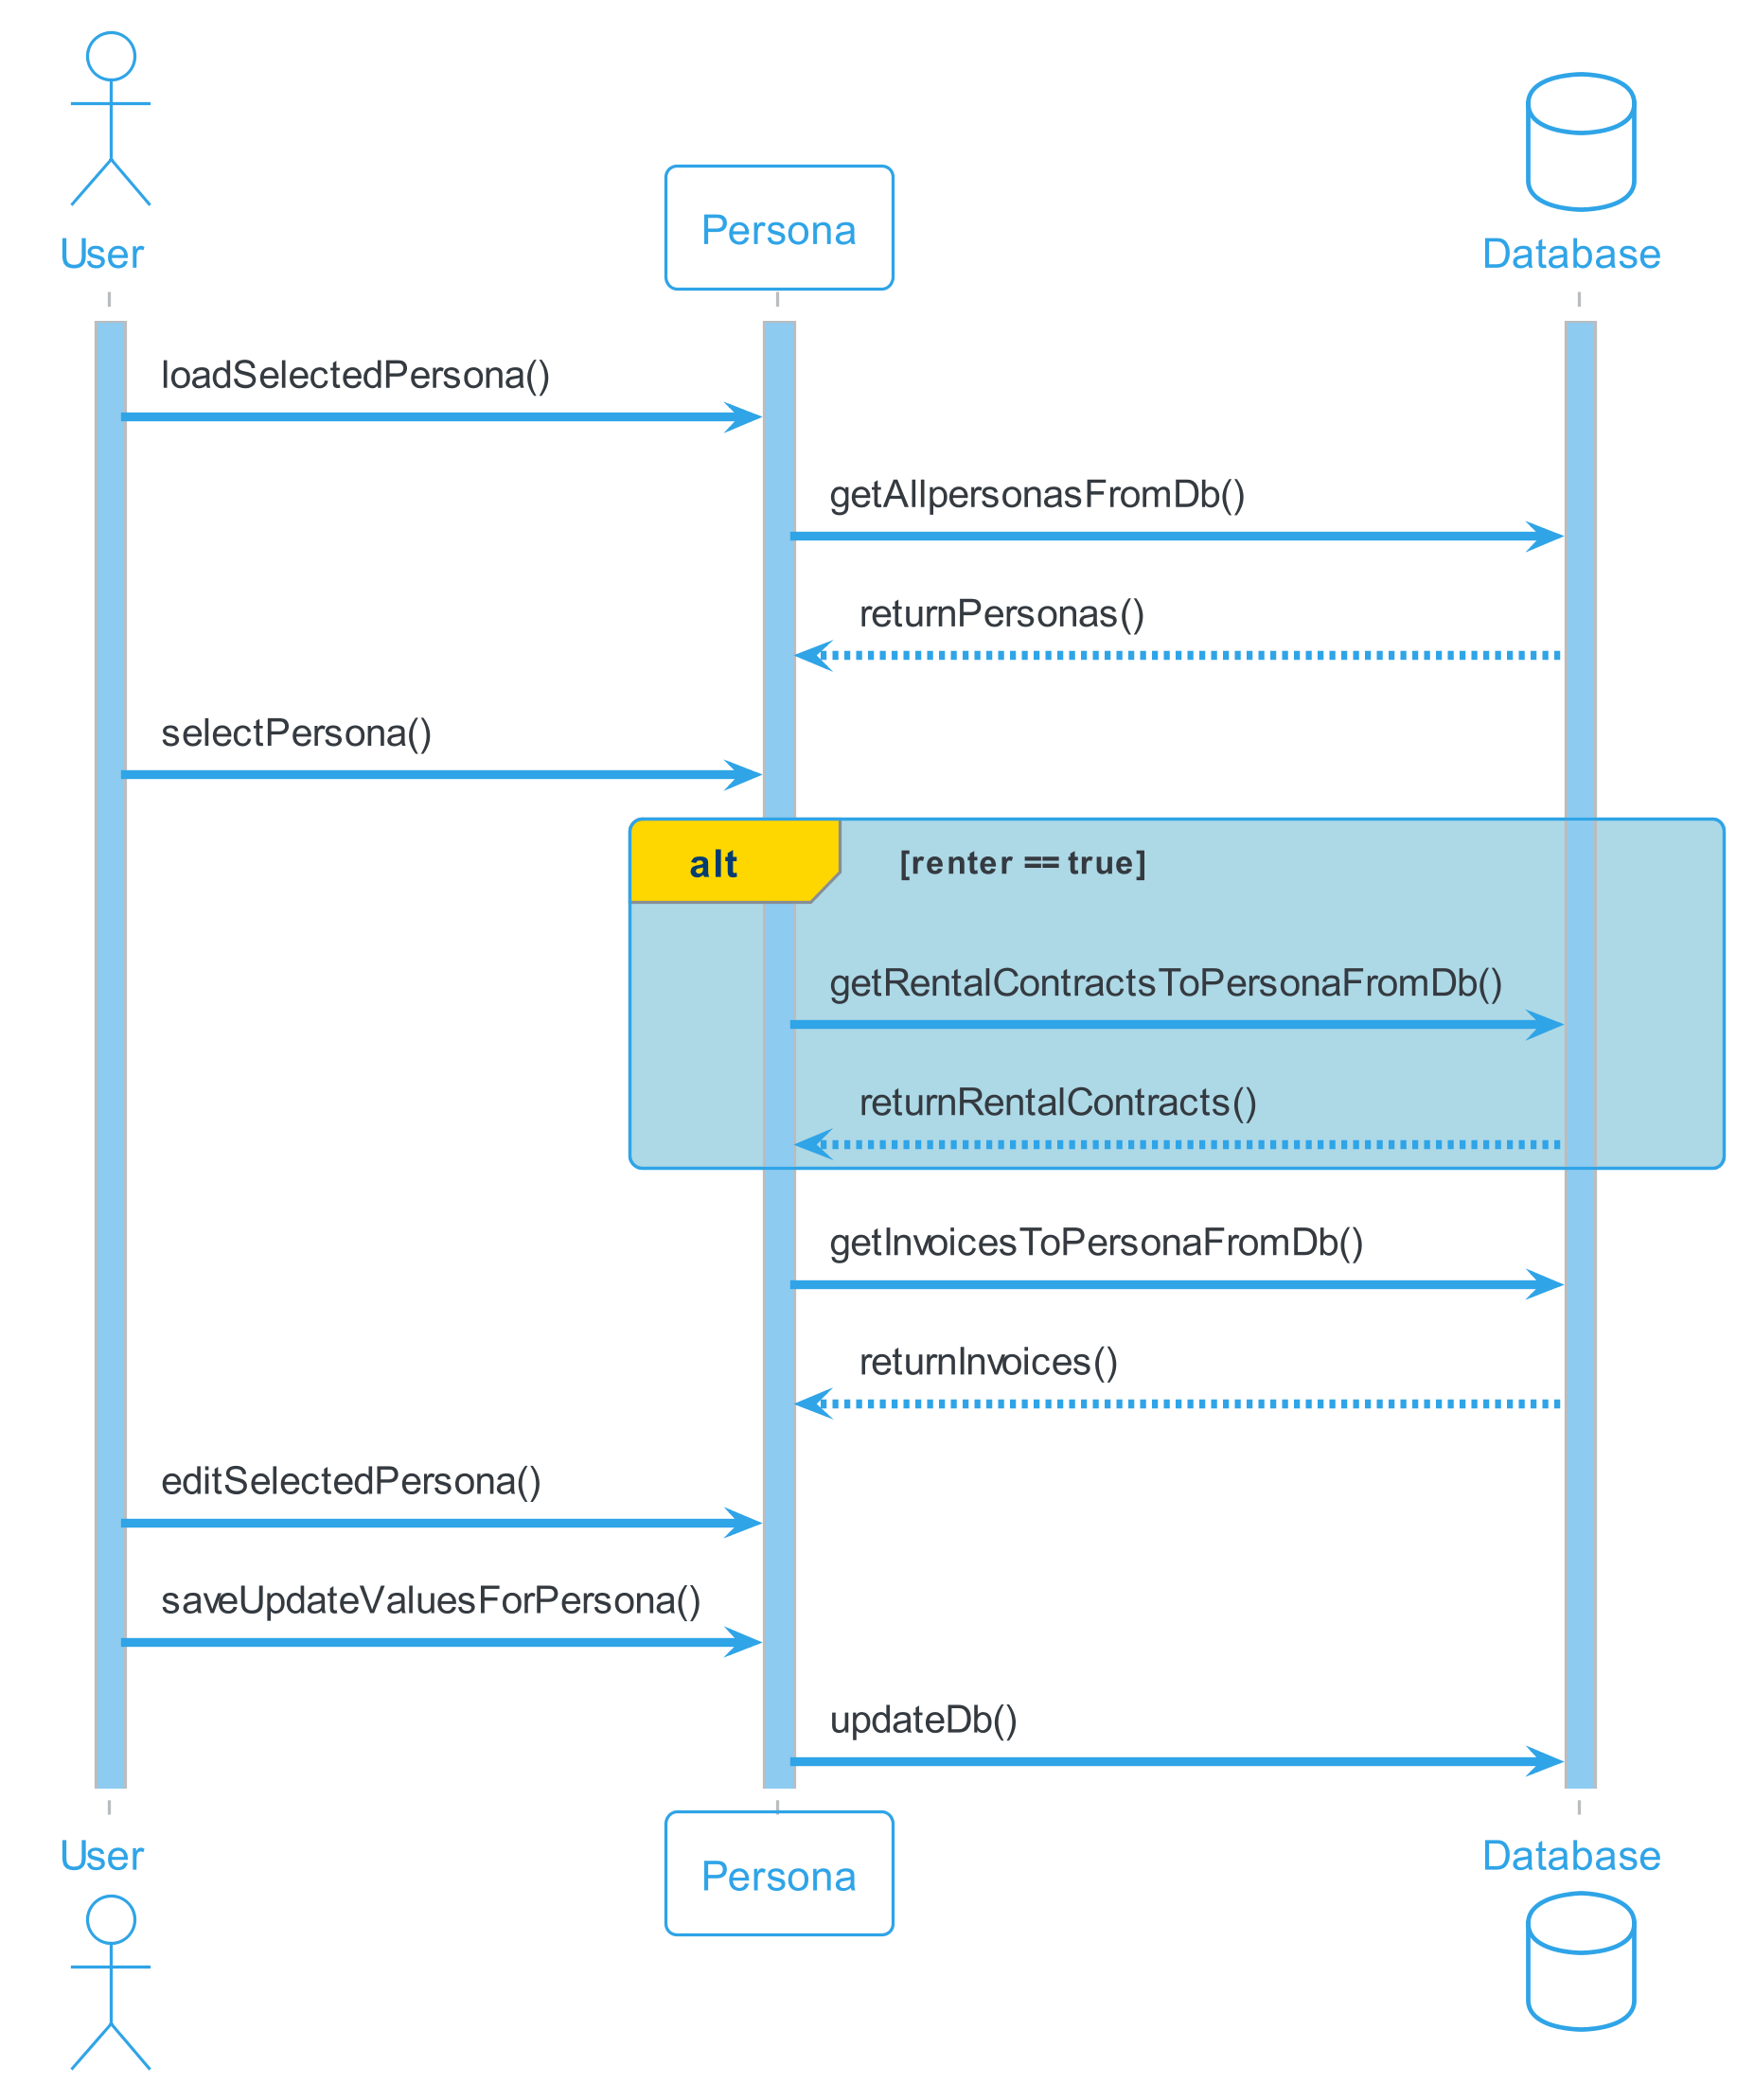
\includegraphics[width=0.7\textheight]{content/diagrams/out/sequenzdiagram/personAnsehen/personAnsehen.png}
    \caption{SQ-Mieter,Kreditor,Hauswart Ansehen / Bearbeiten}
  \end{center}
\end{figure}

\begin{figure}[H]
  \begin{center}
    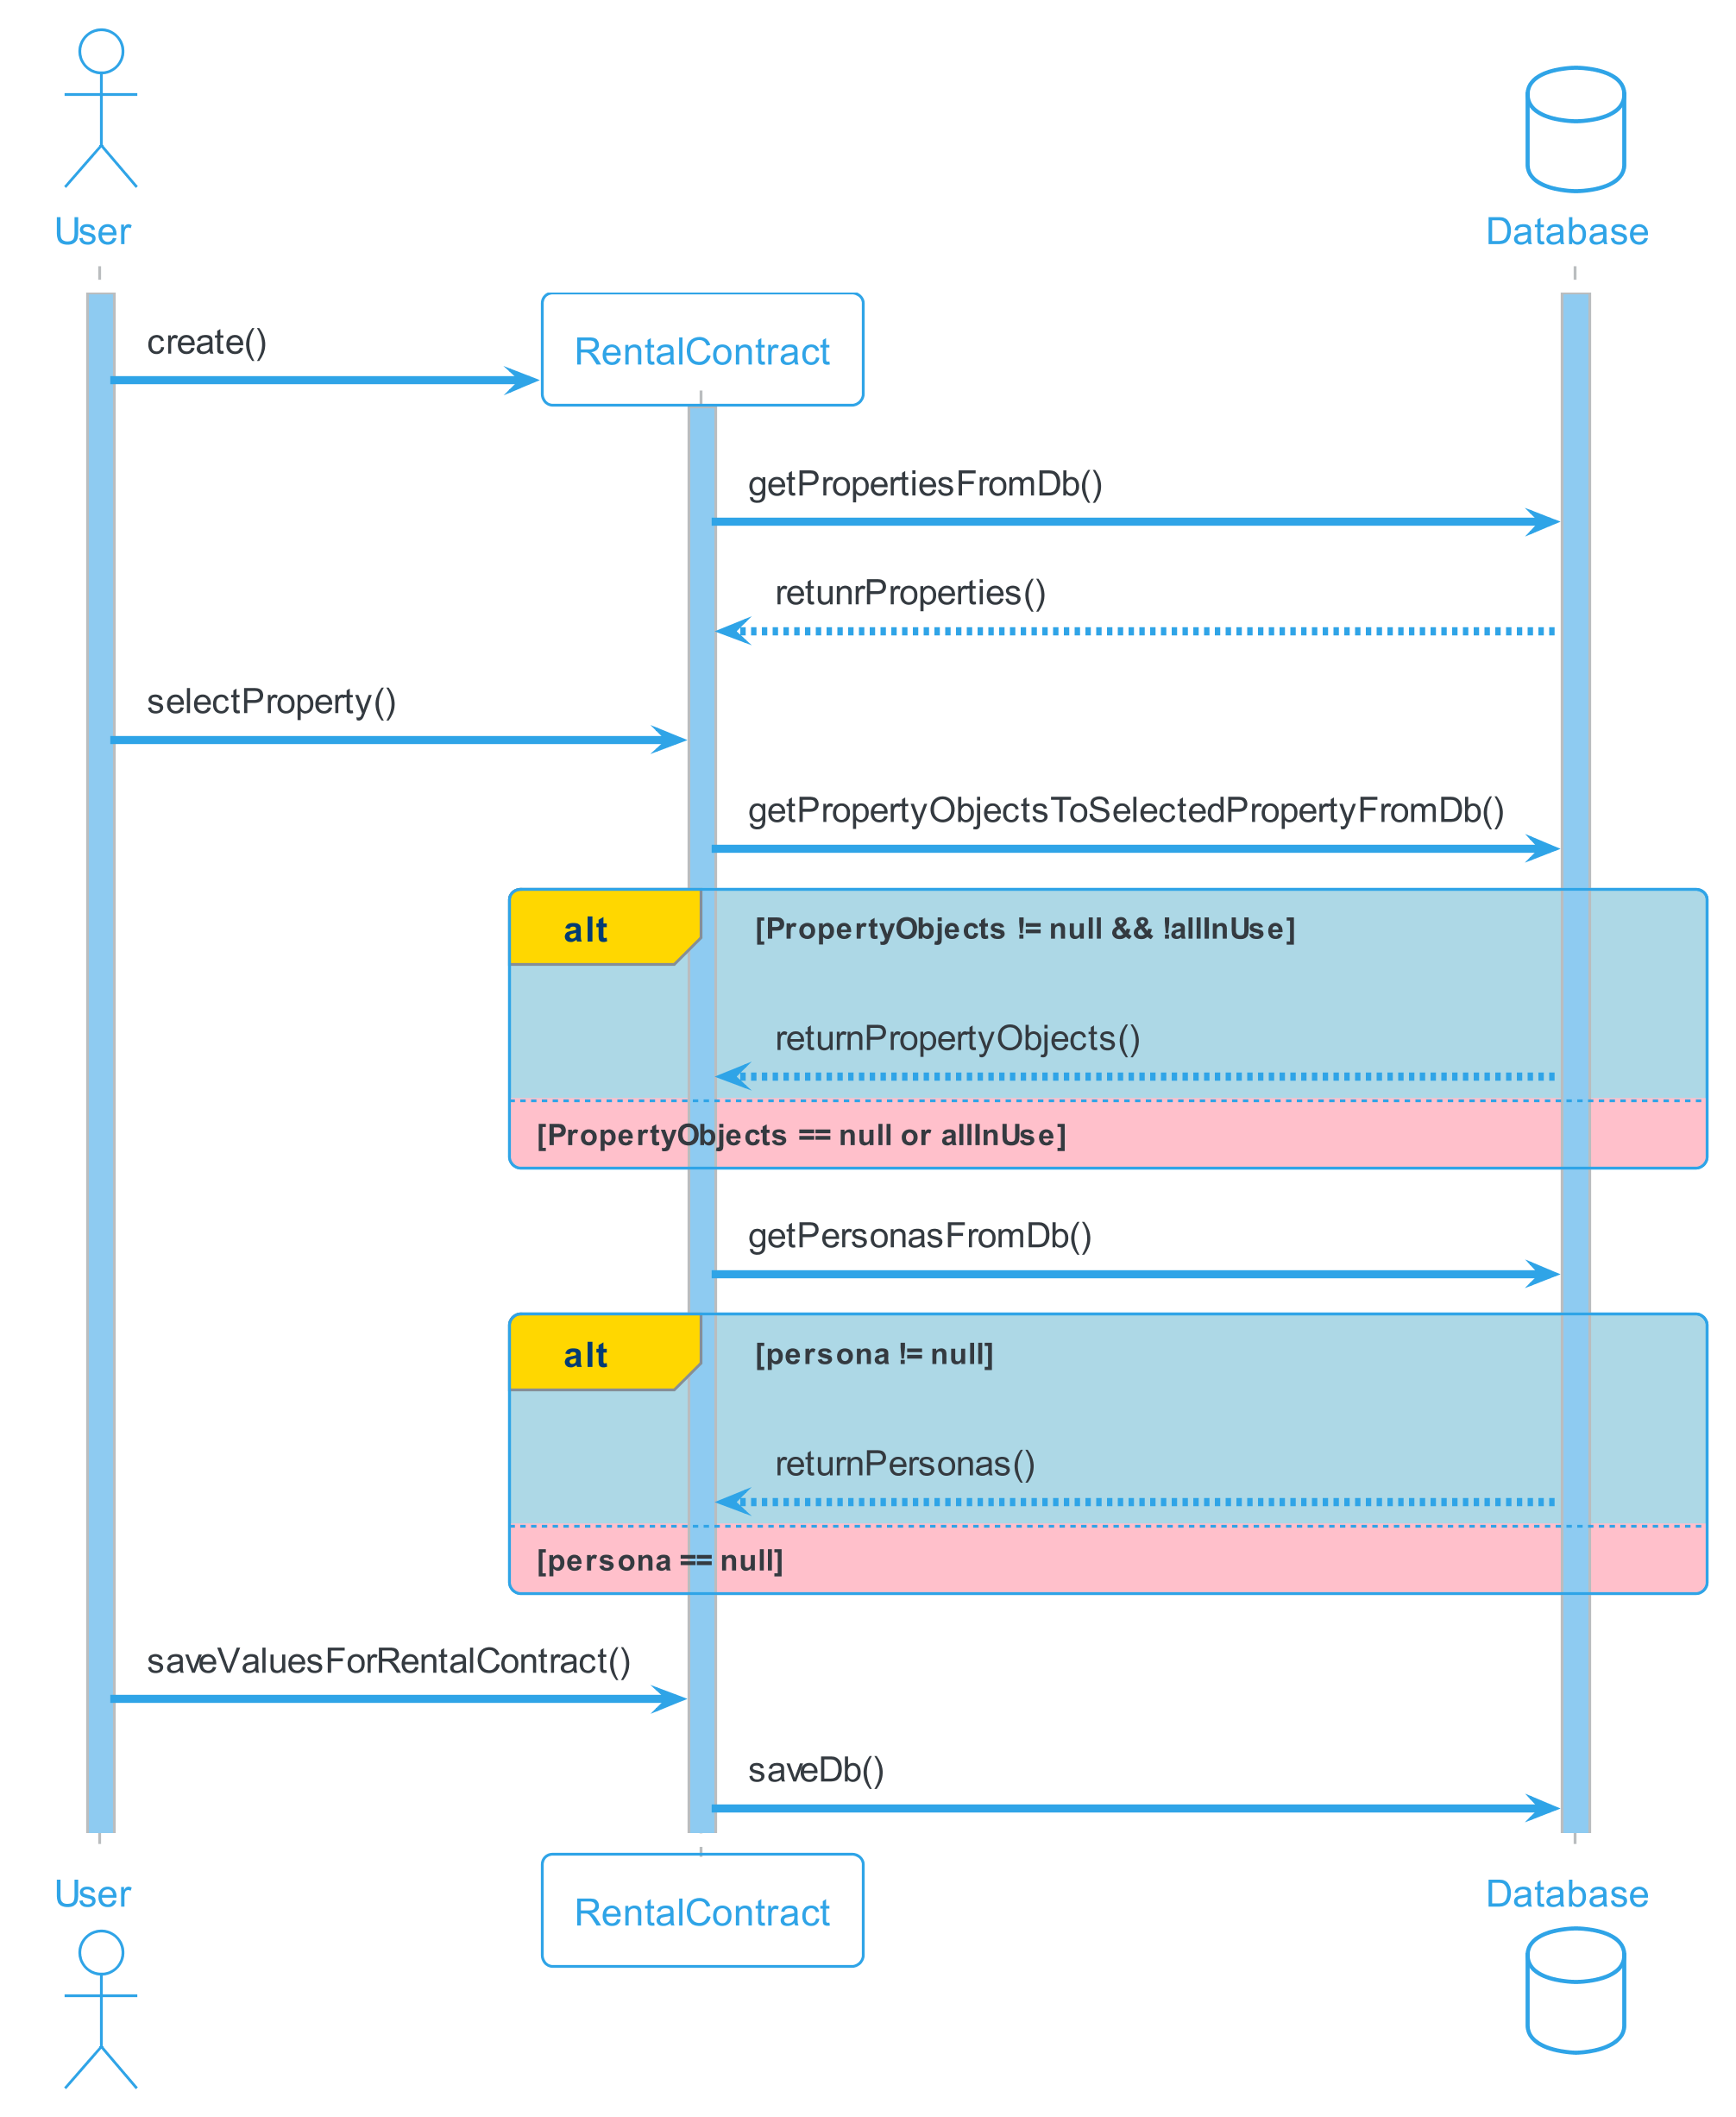
\includegraphics[width=0.9\textwidth]{content/diagrams/out/sequenzdiagram/mietvertrag/mietvertrag.png}
    \caption{SQ-Mietvertrag erstellen}

  \end{center}
\end{figure}

\begin{figure}[H]
  \begin{center}
    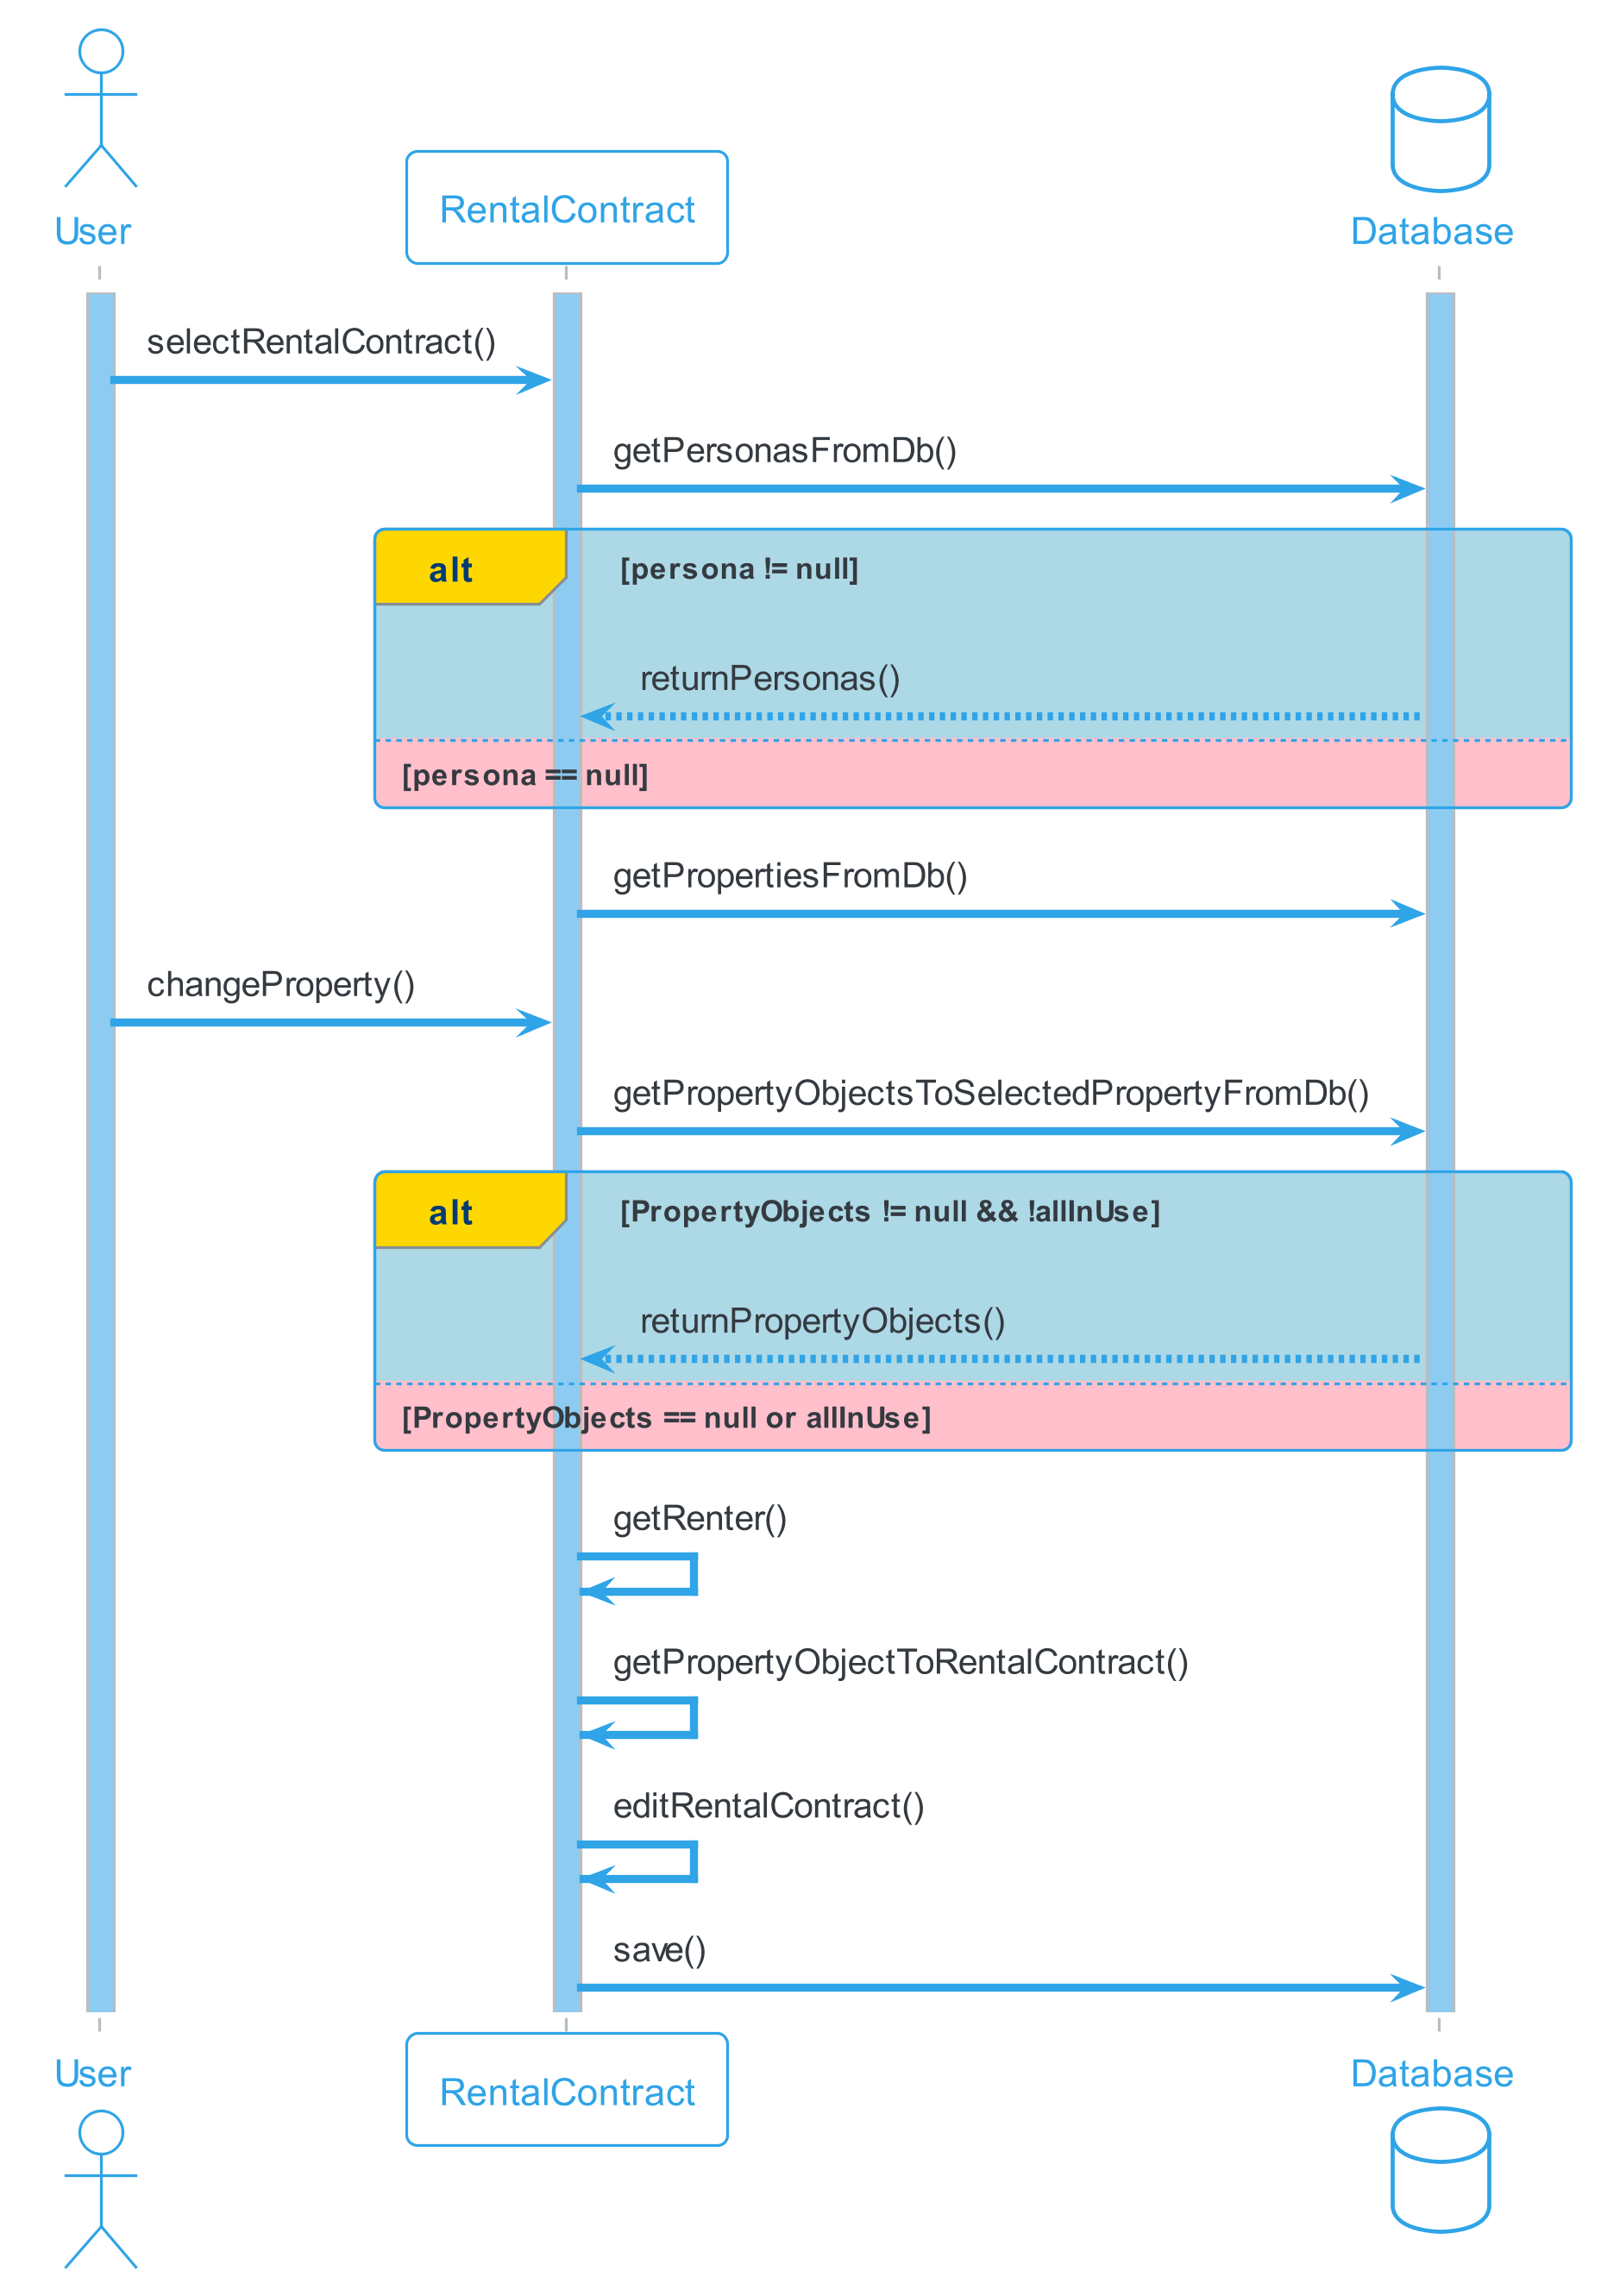
\includegraphics[width=0.6\textheight]{content/diagrams/out/sequenzdiagram/mietvertragEditieren/mietvertragEditieren.png}
    \caption{SQ-Mietvertrag Ansehen / Bearbeiten}

  \end{center}
\end{figure}

\begin{figure}[H]
  \begin{center}
    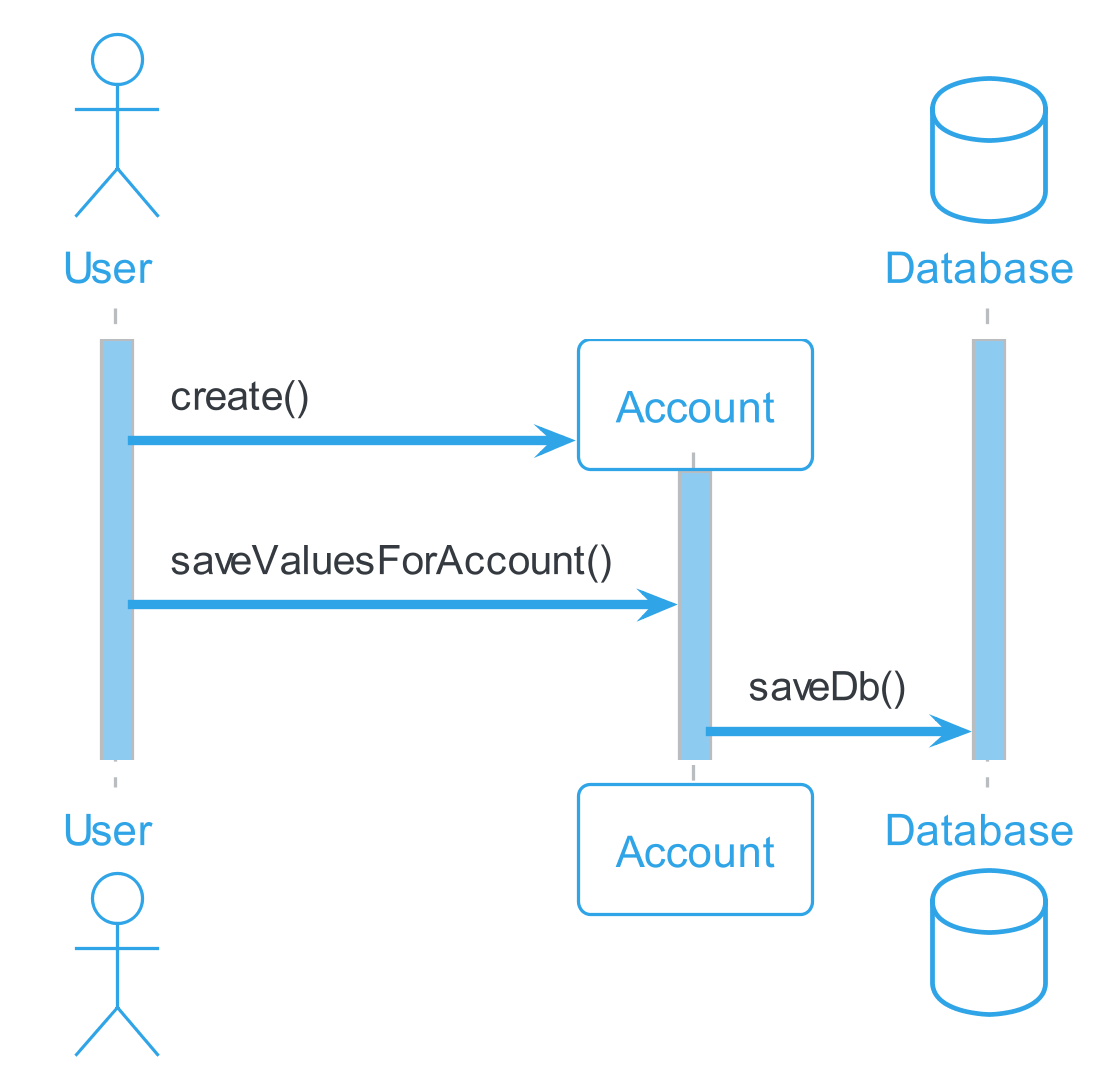
\includegraphics[width=0.5\textheight]{content/diagrams/out/sequenzdiagram/kontoErstellen/KontoErstellen.png}
    \caption{SQ-Konto erstellen}

  \end{center}
\end{figure}

\begin{figure}[H]
  \begin{center}
    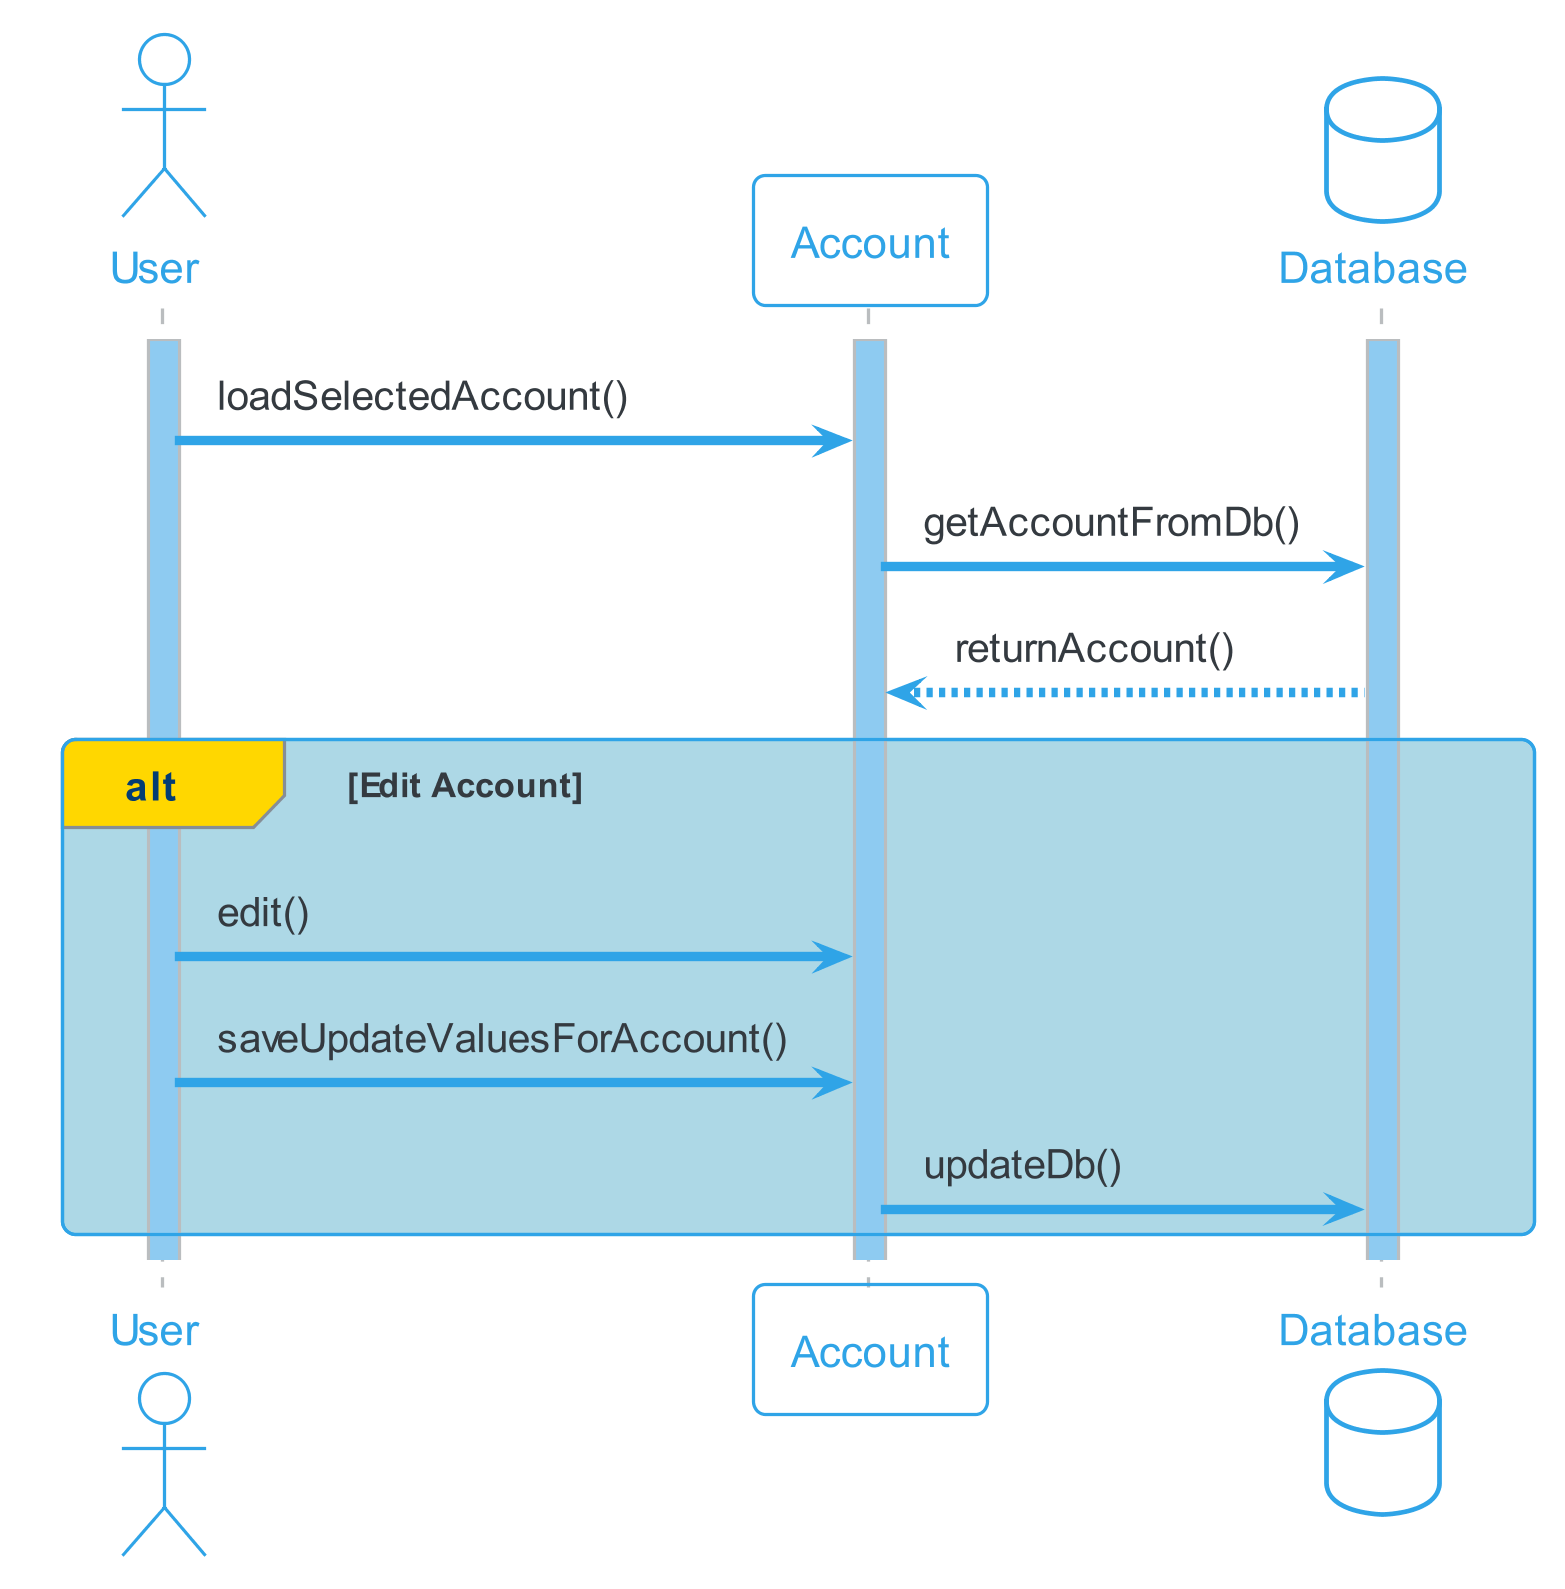
\includegraphics[width=0.65\textheight]{content/diagrams/out/sequenzdiagram/kontoAnsehenBearbeiten/KontoAnsehenBearbeiten.png}
    \caption{SQ-Konto Ansehen / Bearbeiten}
  \end{center}
\end{figure}

\begin{figure}[H]
  \begin{center}
    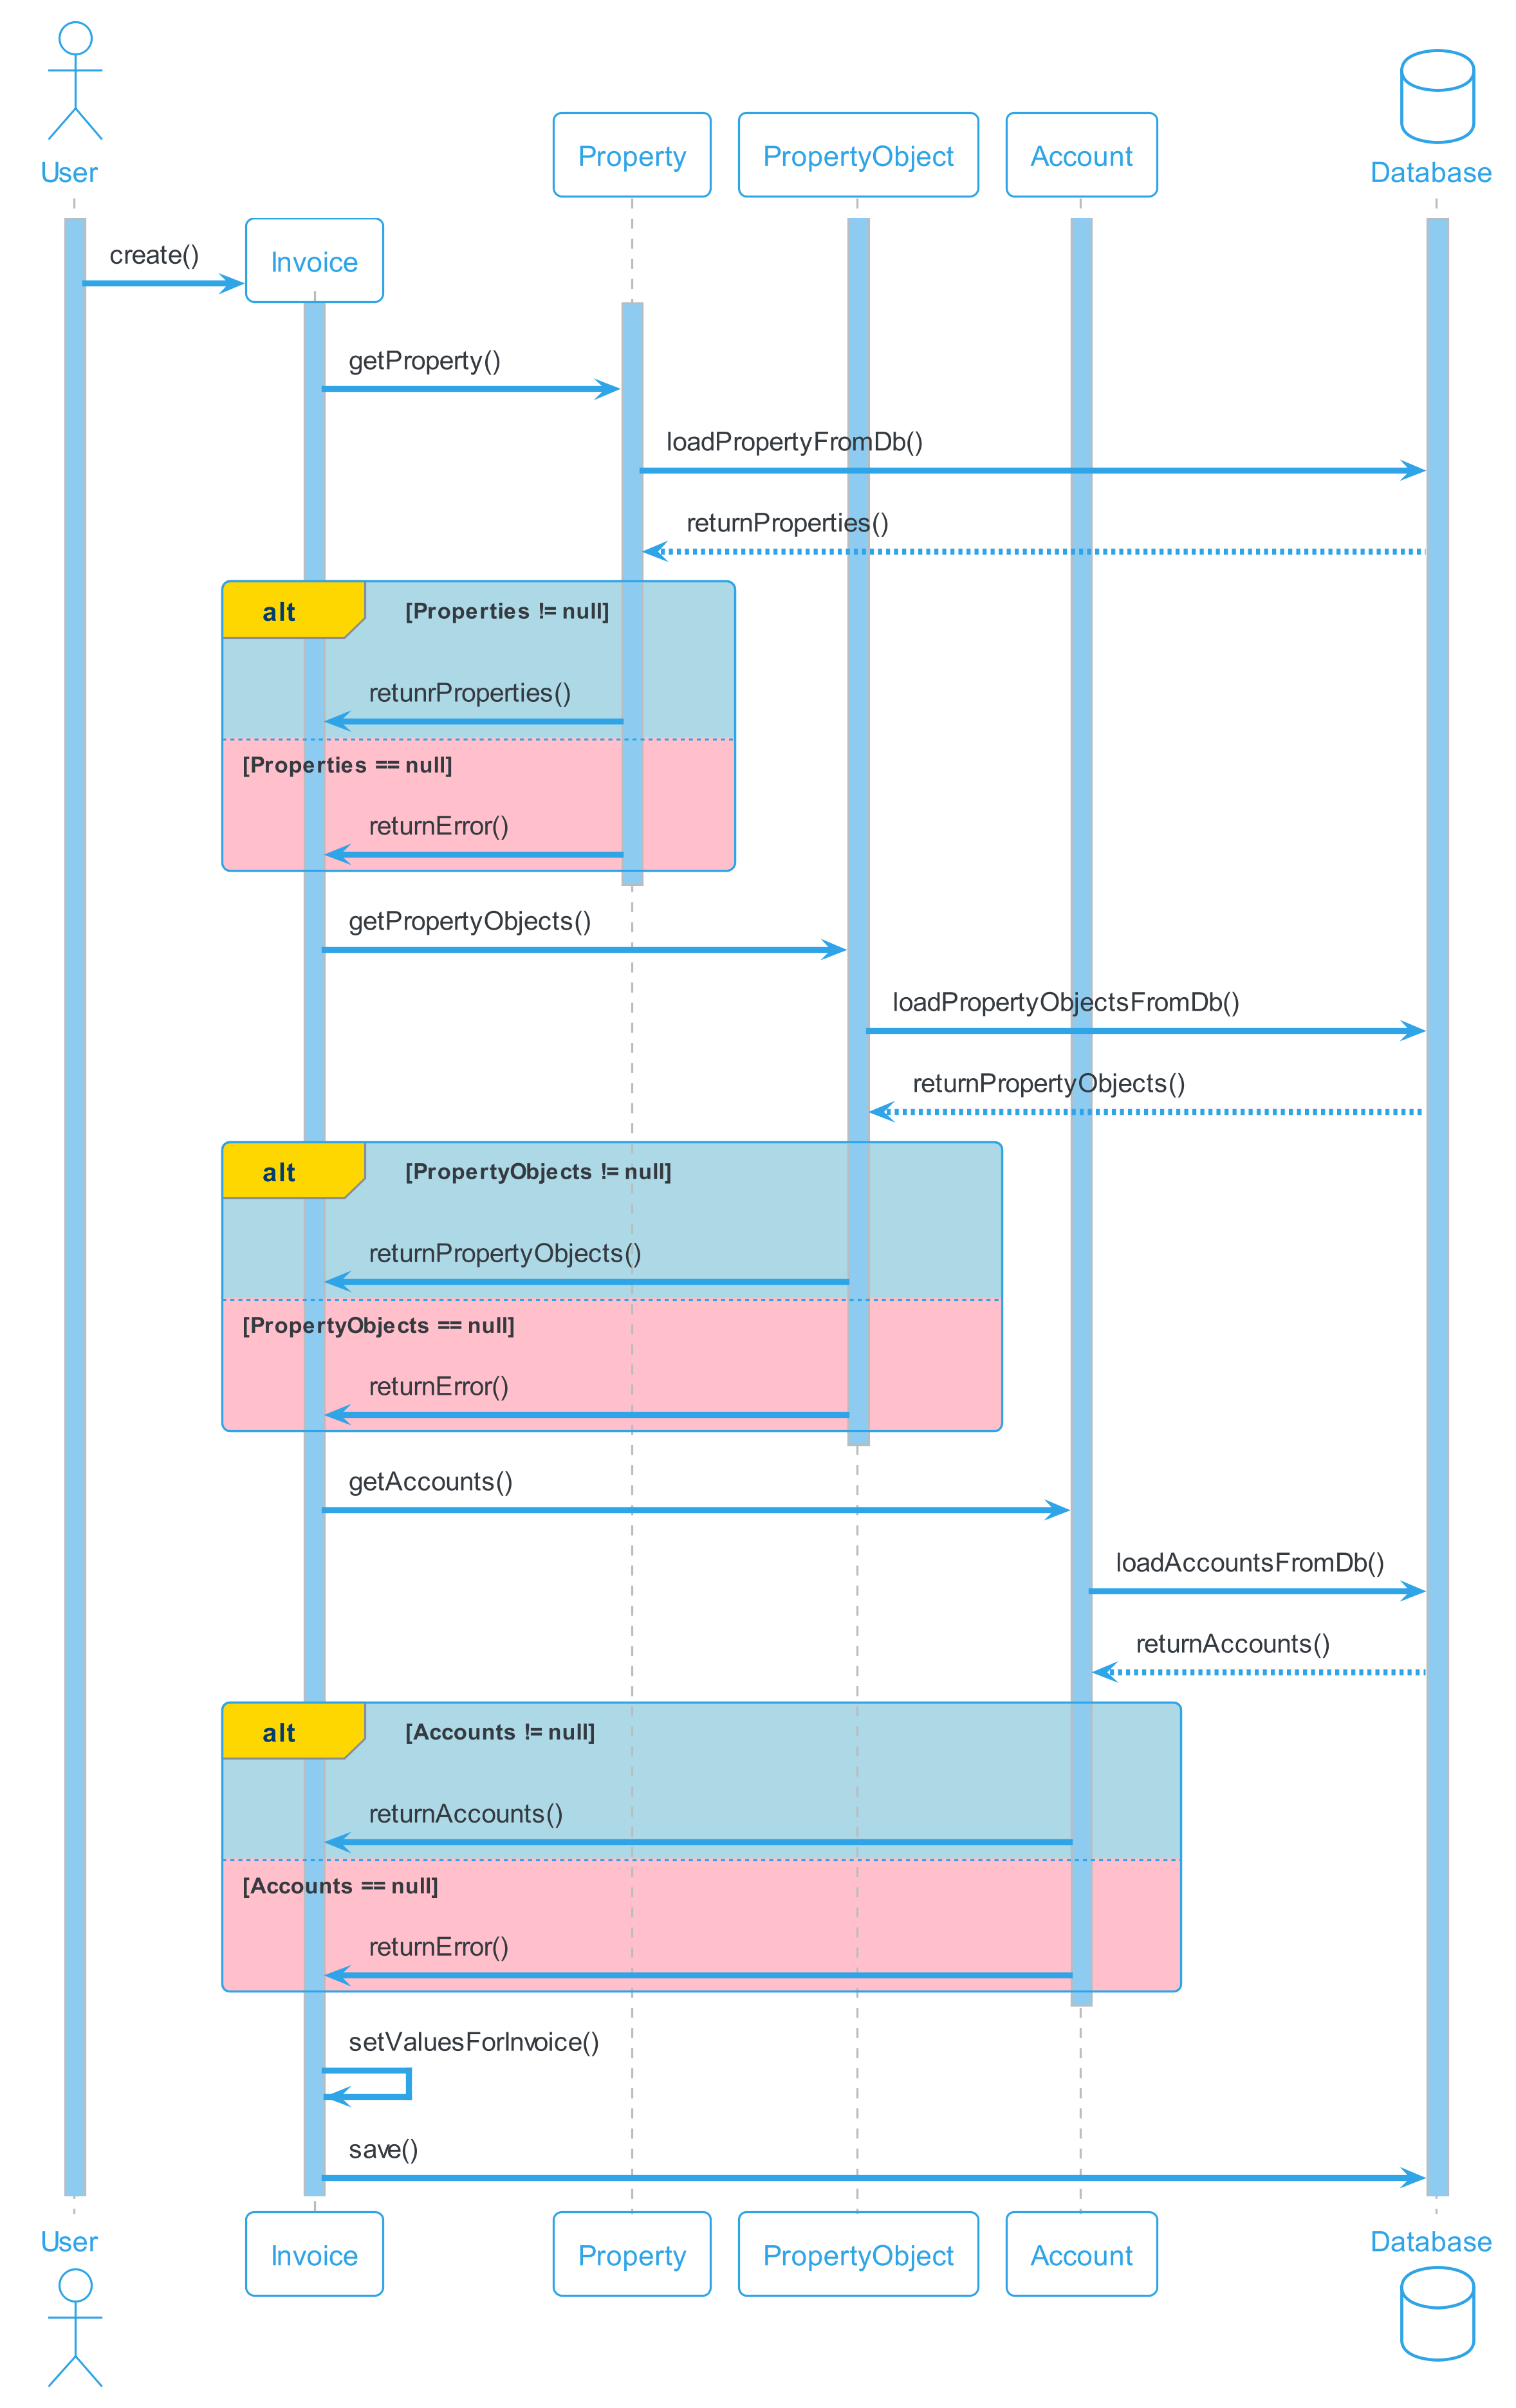
\includegraphics[height=1\textheight]{content/diagrams/out/sequenzdiagram/rechnung/Rechnung.png}
    \caption{SQ-Rechnung}
  \end{center}
\end{figure}